\section{Implemented Features}

\subsection{Infrastructure as Code}

The demo and final solution of this design will be implemented in Terraform through the official AWS provider. Terraform is an Infrastructure as Code (Iac) software tool that allows declarative configuration of cloud infrastructure in a language called Hashicorp Configuration Language (HCL). his allows the management of infrastructure through well known and available tools such as Git, allowing changes to be monitored, strictly confirmed, and rolled back to known working states if necessary. It has extensive documentation available at \url{https://registry.terraform.io/providers/hashicorp/aws/latest/docs}

\subsection{Load Balancing}

To assist in high availability, transparent scaling from an end user perspective, and better access control to elements of the platform, access to the platform will be run through an application load balancer. This sends incoming traffic to multiple targets in multiple availability zones, and monitors the health of those targets. On AWS this feature is called the Elastic Load Balancer (ELB), and scales without administrator input to handle fluctuations in traffic.

A load balancer setup consists of a target group defining protocols, ports, and networks, a group attachment to bind resources to this group, and a listener to apply rules for when to forward traffic. In the Terraform, these are the resources \texttt{aws\_lb\_target\_group}, \texttt{aws\_lb\_target\_group\_attachment}, \texttt{aws\_lb\_listener}, respectively. It is also one of the few resources to belong to a public subnet, so it is publically accessible.

\begin{figure}[H]\label{fig:loadbalancer}
    \centering
    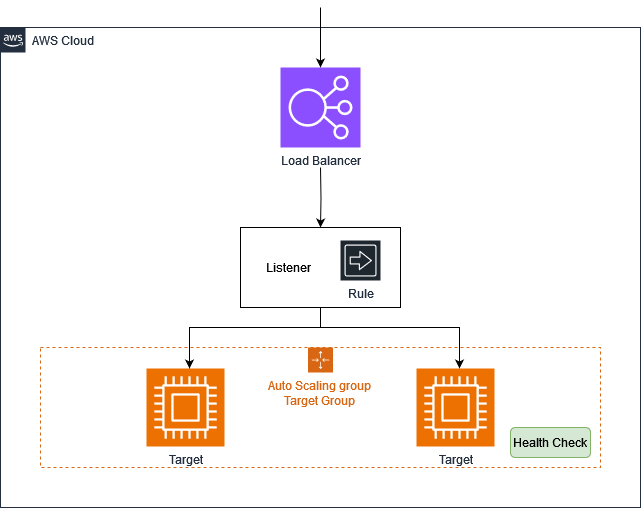
\includegraphics[width=.8\textwidth]{loadbalancer}
    \caption{Example Load Balancer Topology}
\end{figure}

\subsection{Scaling (Compute)}

Using EC2 autoscaling groups, AWS will launch new compute instances as demand increases on pre-existing ones, placing them behind the ALB. Retaining a minimum of 1 instance ensures constant availability. An option available is keep ``warm pools'' of compute instances pre-initialized but not in use, allowing near instant upscaling as demand spikes, though it is not implemented in this solution.

\subsection{High Availability}

High availability will be achieved through seperating cloud resources across two AWS availability zones (AZs), allowing an entire region of AWS to lose access, while maintaining service for customers. It also allows upgrades to infrastructure and software to cause a temporary planned outage in one region while maintaining uninterrupted service globally.

\subsection{Backups}

EBS snapshots are copies of compute drives at a point in time for some EC2 instance. These allow the restoration of an EC2 as it was at that point in time without much friction. These are critical as a lot of the work performed on EC2s will be with ephemeral data that is critical to a user's experience. If a compute instance were to go down, this information can be restored without much delay \autocite{amazonwebservicesAmazonEBS2023}.

RDS backups occur daily in a specified time controlled by AWS. This ensures that critical user data is intentionally redundant. Alongside this is a read-only instance replica. This ensures that the load on the primary DB is never too excessive, and access is always available even when heavy writes are underway. Ideally, there would also be a third standby replica, where no client has read access at all. This will be in place to ensure further redundancy and backups. It will not be implemented in the demo, but planned and accounted for in the design \autocite{amazonwebservicesEncryptingAmazonRDS2023}.

S3 is an extremely simple service to use, and promises four 9s of availability and eleven 9s of object durability. This is done by distributing and cloning obejcts across multiple availability zones without the need for administrator input \autocite{amazonwebservicesAmazonSimpleStorage2023}.
